\section{Projeto de Pontes de Madeira}\label{sec:ponte_madeira}

As pontes de madeira, uma das formas mais antigas de estrutura de travessia, evoluíram significativamente em sua concepção e aplicação.
Atualmente, podem ser classificadas em diversos tipos estruturais, cada um com suas particularidades, vantagens e contextos de aplicação adequados.
O objetivo desta seção é apresentar alguns modelos de pontes de madeira e particularidades de dimensionamento.

\subsection{Tipologias de pontes de madeiras}

As tipologias de pontes de madeira são as mais variadas possíveis e, neste trabalho, serão apresentados apenas modelos de pontes de madeira em viga.
Segundo a classificação proposta por \textcite{ritter1990}, as superestruturas em viga podem ser subdivididas nos seguintes tipos:
\begin{itemize}
    \item vigas de toras roliças (\textit{log beams});
    \item vigas de madeira serrada (\textit{sawn lumber beams});
    \item vigas de madeira laminada colada (\textit{glued-laminated timber beams} -- MLC);
    \item vigas de madeira laminada colada de lâminas paralelas (\textit{laminated veneer lumber beams} -- LVL).
\end{itemize}


\begin{figure}[htpb!]
    \centering

  % primeira imagem
    \begin{minipage}[t]{0.45\textwidth}
        \centering
        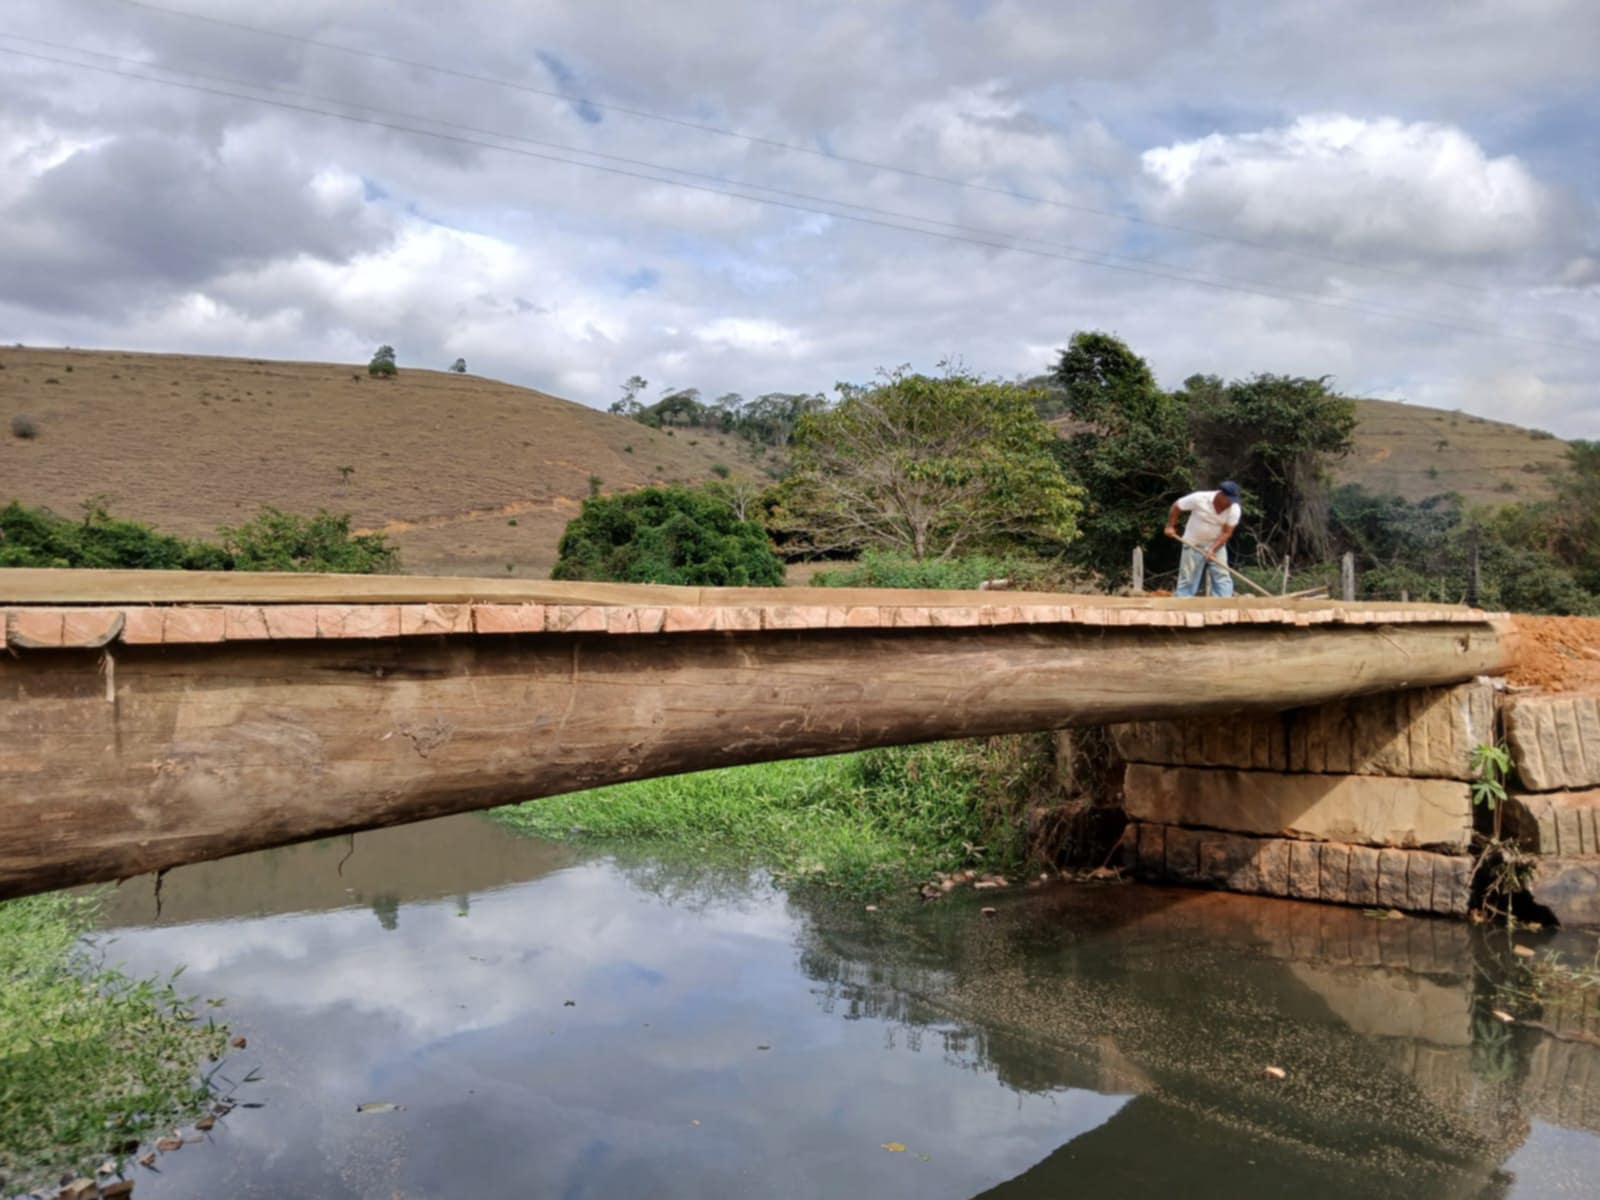
\includegraphics[width=\textwidth]{figuras/pontenativa.jpg}
    \end{minipage}
     % segunda imagem
    \begin{minipage}[t]{0.45\textwidth}
        \centering
        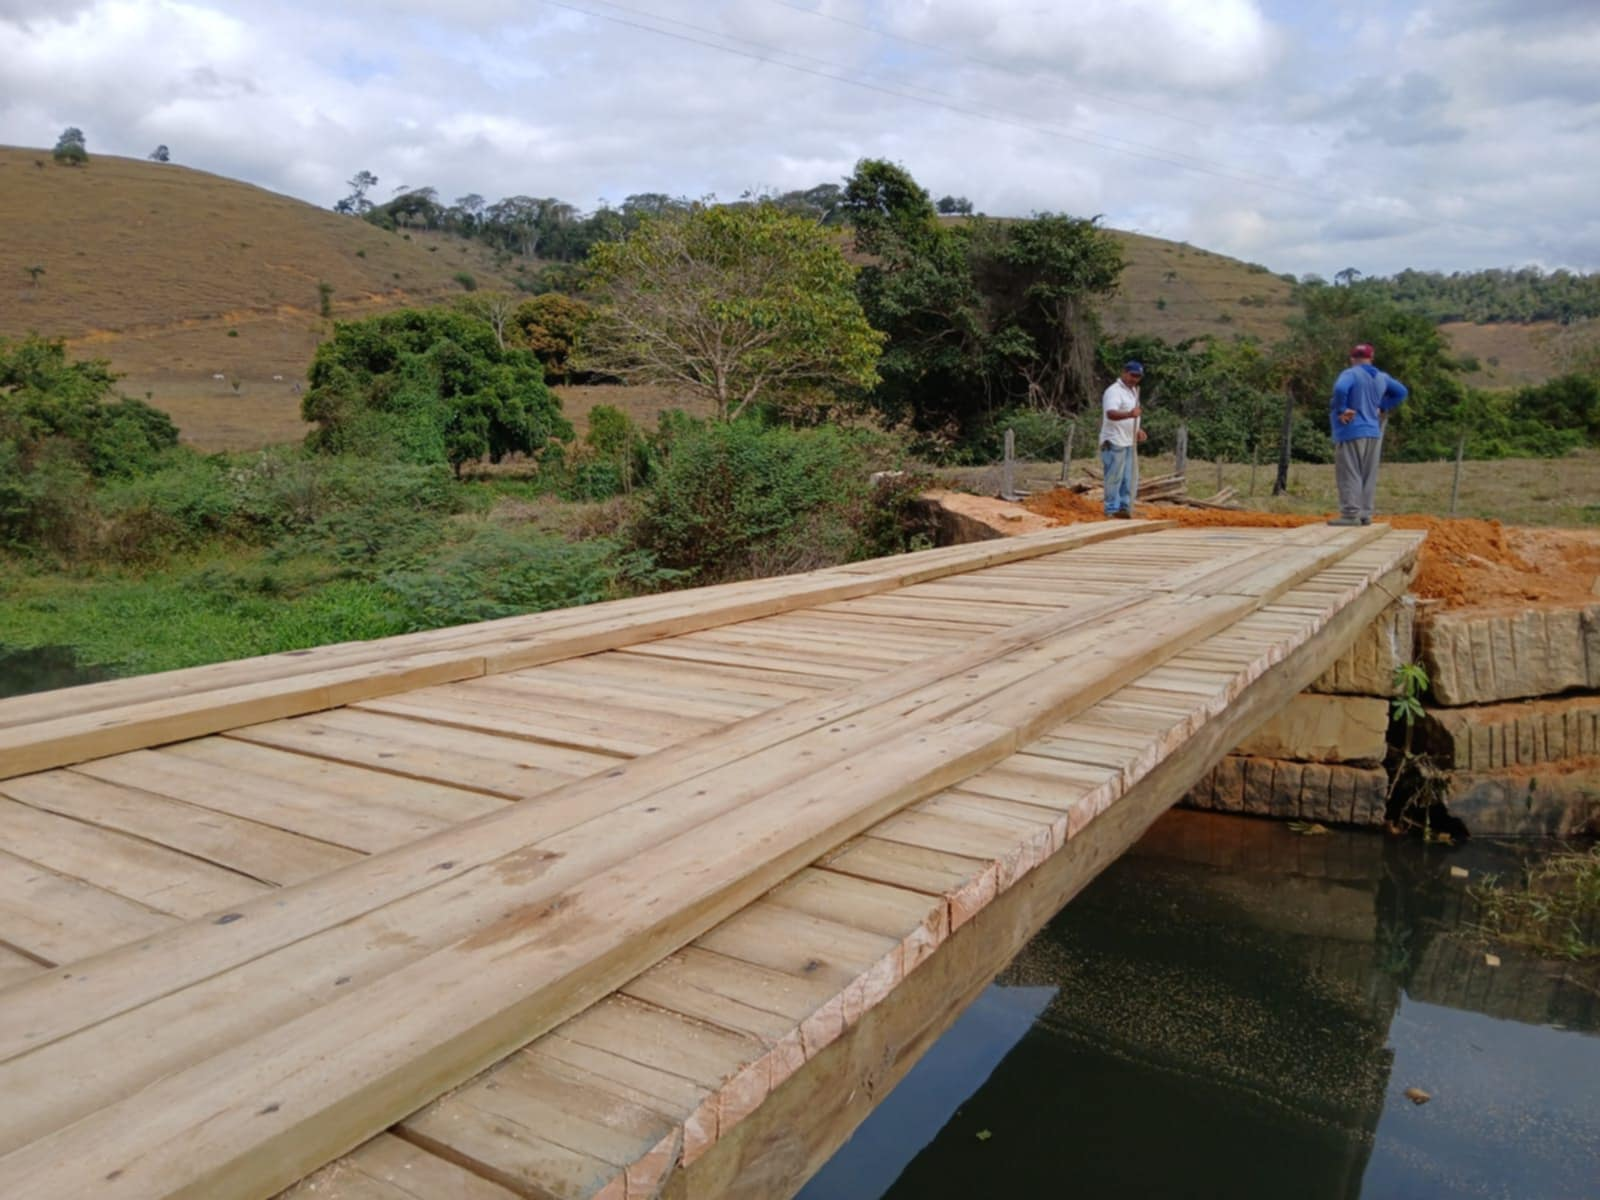
\includegraphics[width=\textwidth]{figuras/pontenativa2.jpg}
    \end{minipage}
    \caption{Ponte de madeira nativa roliças sobre Córrego do Ouro \parencite{gazeta2025ponte}.}
    \label{fig:pontenat}
\end{figure}

A Figura \ref{fig:pontenat} apresenta exemplos de pontes de madeira que são comumente encontradas
em regiões de estradas vicinais do Brasil. A ponte exemplificada consiste em uma ponte rural de pequeno porte, construída predominantemente em madeira, com sistema estrutural em viga de toras roliças apoiadas em fundação superficiais nas margens do córrego. Sobre as vigas é instalado o tabuleiro de pranchas, complementado por pranchas longitudinais formando o rodeiro sob a linha das rodas dos veículos. O conjunto também necessita de elementos de travamento e fixação, como parafusos, pregos, barras ou chapas, garantindo a estabilidade e a união entre as peças. Dessa forma, o caminho das cargas ocorre do veículo para o tabuleiro, do tabuleiro para as vigas e, posteriormente, para os apoios e o terreno.

Segundo \textcite{ritter1990}, a extensão do vão, em pontes de toras roliças, depende da espécie, diâmetro e
comprimento das árvores disponíveis.
Vãos frequentes variam entre 6 e 18 metros, mas há exemplares documentados que se aproximam dos 30 metros, capazes de suportar
veículos com carga total superior a 100 toneladas.

\subsection{Diâmetro das toras roliças}

Para o dimensionamento de peças de seção circular variável, como toras roliças, adota-se um diâmetro equivalente de cálculo, $d_{eq}$, conforme o item 9.7 da \textcite{NBR7190-1:2022}, correspondente ao diâmetro da seção localizada a $1/3$ do comprimento total da peça, medido a partir da extremidade de menor diâmetro conforme a figura \ref{fig:dequivalente}. Dessa forma, considera-se a peça como tendo seção uniforme ao longo de seu comprimento, adotando-se o diâmetro obtido nessa posição.

Entretanto, o valor de $d_{eq}$ é limitado a, no máximo, $1,5$ vezes o diâmetro da extremidade mais delgada, $d_2$. Assim, o diâmetro equivalente pode ser determinado por:

\begin{equation}
d_{eq} = d_2 + \frac{d_1-d_2}{3}
\end{equation}

devendo ser respeitada a seguinte condição:

\begin{equation}
d_{eq} \leq 1,5d_2
\end{equation}

onde $d_1$ corresponde ao maior diâmetro da tora, $d_2$ ao menor diâmetro e $L$ ao comprimento total da peça.

\begin{figure}[htpb!]
\centering
\begin{tikzpicture}[
  dim/.style={<->, >={Latex[length=2mm]}, thin},
  every node/.style={font=\footnotesize}
]
% geometria (evitar \L -- e o comando reservado do LaTeX para "L-slash")
\pgfmathsetmacro{\Ltot}{6}
\pgfmathsetmacro{\rTwo}{0.4}
\pgfmathsetmacro{\rOne}{0.9}
\pgfmathsetmacro{\xEq}{2}
\pgfmathsetmacro{\rEq}{\rTwo + (\rOne-\rTwo)*(\xEq/\Ltot)}
\pgfmathsetmacro{\xMidA}{\xEq/2}
\pgfmathsetmacro{\xMidB}{\xEq + (\Ltot-\xEq)/2}
\pgfmathsetmacro{\xMidL}{\Ltot/2}

% ---- corpo afunilado da tora ----
\draw[thick] (0,\rTwo) -- (\Ltot,\rOne);
\draw[thick] (0,-\rTwo) -- (\Ltot,-\rOne);
\draw[thick] (0,0) ellipse [x radius=0.12, y radius=\rTwo];
\draw[thick] (\Ltot,0) ellipse [x radius=0.18, y radius=\rOne];

% ---- plano de medicao do deq ----
\draw[dash dot, thin] (\xEq,-\rEq-0.15) -- (\xEq,\rEq+0.15);

% ---- cotas verticais ----
\draw[dim] (-0.9,-\rTwo) -- (-0.9,\rTwo);
\node at (-1.25,0) {$d_2$};

\draw[dim] (\xEq,-\rEq) -- (\xEq,\rEq);
\node at (\xEq+0.45,0) {$d_{eq}$};

\draw[dim] (\Ltot+0.9,-\rOne) -- (\Ltot+0.9,\rOne);
\node at (\Ltot+1.25,0) {$d_1$};

% ---- cotas horizontais ----
\draw[dim] (0,-\rOne-0.7) -- (\xEq,-\rOne-0.7);
\node at (\xMidA,-\rOne-0.95) {$L/3$};

\draw[dim] (\xEq,-\rOne-0.7) -- (\Ltot,-\rOne-0.7);
\node at (\xMidB,-\rOne-0.95) {$2L/3$};

\draw[dim] (0,-\rOne-1.4) -- (\Ltot,-\rOne-1.4);
\node at (\xMidL,-\rOne-1.65) {$L$};
\end{tikzpicture}
\caption{Diâmetro Equivalente \parencite{NBR7190-1:2022}.}
\label{fig:dequivalente}
\end{figure}

Esse critério permite representar uma peça de seção circular variável por uma seção uniforme equivalente para fins de dimensionamento estrutural.




% \begin{fillblock}
% Descrever o critério de determinação do diâmetro equivalente da tora roliça (por exemplo, diâmetro na seção correspondente a 1/3 do comprimento da peça a partir da extremidade de maior diâmetro). Incluir figura esquemática com o diâmetro mínimo, médio e equivalente ao longo do comprimento da peça (arquivo a salvar em \texttt{figuras/}).
% \end{fillblock}

\subsection{Carga do trem tipo}\label{sec:trem_tipo}

As cargas delimitadas nas pontes brasileiras são definidas pela \textcite{nbr7188}, que estabelece
os requisitos para o projeto de pontes rodoviárias. A norma apresenta dois modelos de trem-tipo para uso: o TB-450 e o TB-240. Porém, por se tratar de estradas vicinais,
serão contemplados apenas os detalhes do TB-240.
Esse trem-tipo é caracterizado por um veículo de 240 kN de peso total, constituído por seis rodas e três eixos.
Cada eixo do veículo aplica uma carga de 40 kN, com espaçamentos de 1,5 m entre os eixos.
A área de ocupação do veículo deve ser de 18,0 m², complementada por uma carga
uniformemente distribuída de 4,0 kN/m² em seu entorno (multidão), conforme a Figura \ref{fig:trem}.

\begin{figure}[htpb!]
\centering
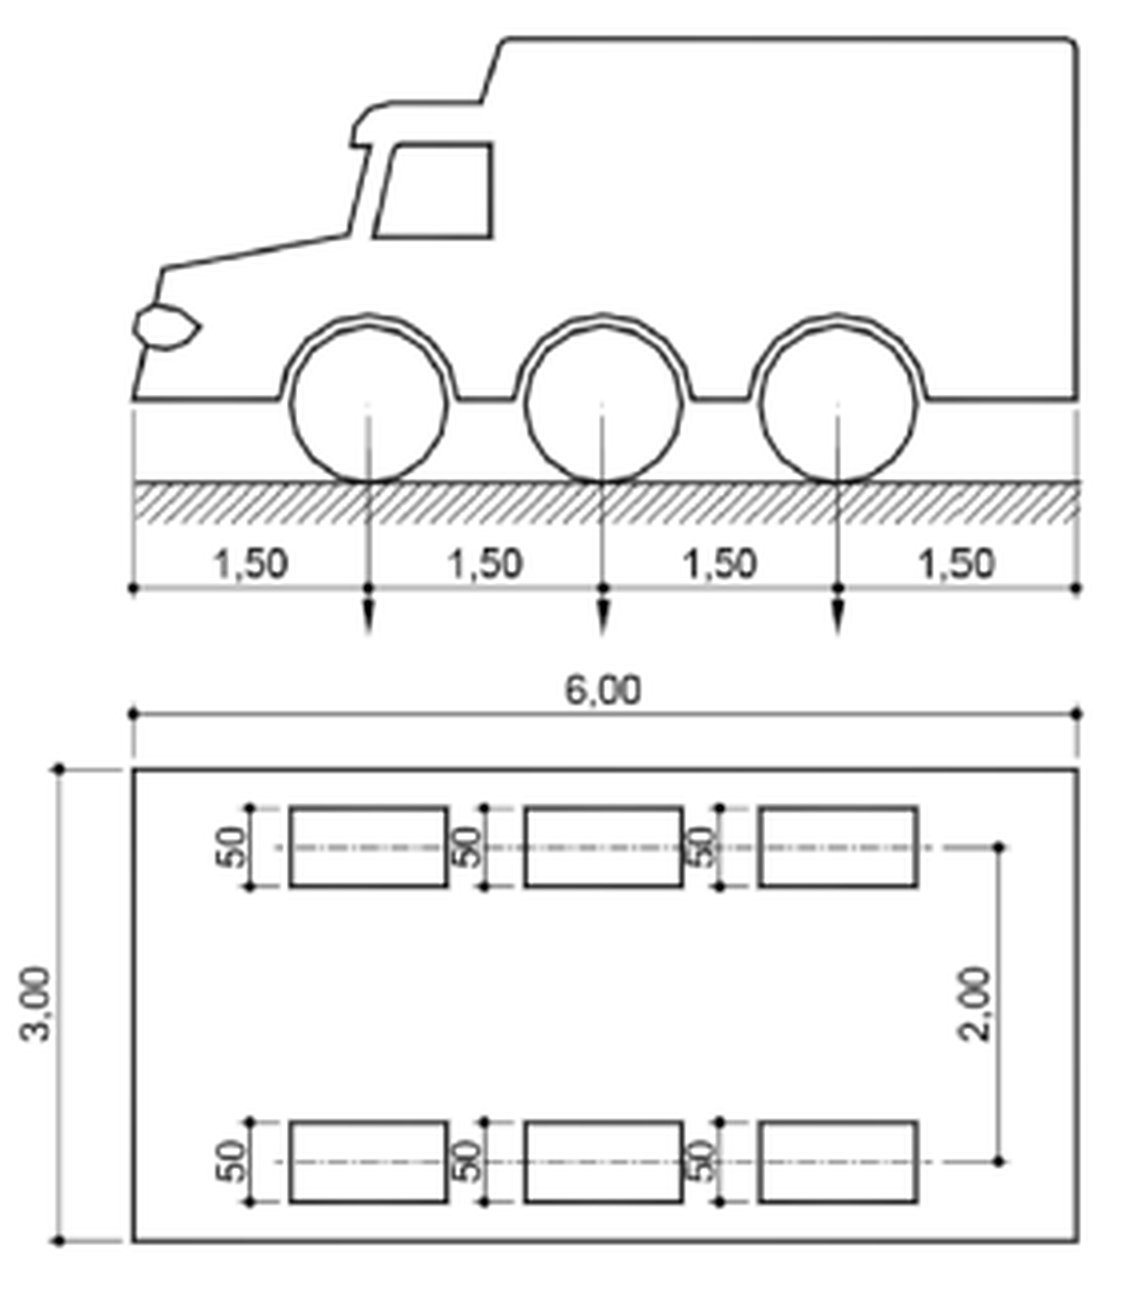
\includegraphics[width=0.4\textwidth]{figuras/trem1_hq.png}
\caption{Configuração trem de tipo \parencite{nbr7188}.}
\label{fig:trem}
\end{figure}

\subsection{Propriedades da Madeira}

\subsubsection{Anatomia, fisiologia e comportamento mecânico da madeira}
\label{sec:anatomia_madeira}

A compreensão do comportamento estrutural da madeira parte de sua organização anatômica e das funções que desempenha na árvore viva.
A madeira corresponde ao xilema secundário, tecido associado à condução de água e nutrientes minerais, ao armazenamento de substâncias e à sustentação da planta.
Seu crescimento em espessura decorre da atividade do câmbio vascular, que produz xilema para o interior e floema para o exterior do tronco \parencite{WiedenhoeftEberhardt2021}.

Na seção transversal do tronco, distinguem-se medula, cerne, alburno, região cambial e cascas, conforme a Figura~\ref{fig:anatomia_madeira}.
A medula ocupa a região central e está associada ao desenvolvimento inicial do caule.
O alburno constitui a porção condutora do xilema e também participa do armazenamento de reservas, enquanto o cerne corresponde à região interna que perdeu a função de condução de água e pode acumular extrativos.
A casca interna, ou floema, transporta produtos da fotossíntese; a casca externa protege os tecidos internos.
Os raios contribuem para o transporte radial e o armazenamento de substâncias \parencite{WiedenhoeftEberhardt2021}.

\begin{figure}[htbp]
\centering
% Esquema vetorial original; proporções didáticas, sem escala.
% Seção do tronco com setor removido e detalhe celular de uma conífera.
\begin{tikzpicture}[
  x=1cm,y=1cm,
  every node/.style={font=\footnotesize},
  chamada/.style={thin,draw=black!75},
  contorno/.style={draw=black!80,line width=0.55pt}
]
\def\topo{2.6}
\def\altura{3.3}
\def\achatamento{0.43}

% Casca: superfícies externas visíveis do tronco.
\foreach \inicio/\fim in {180/290,345/360} {
  \path[contorno,fill=black!32]
    ({2.8*cos(\inicio)},{\topo+2.8*\achatamento*sin(\inicio)})
    arc[start angle=\inicio,end angle=\fim,x radius=2.8,y radius=1.204]
    -- ({2.8*cos(\fim)},{\topo-\altura+2.8*\achatamento*sin(\fim)})
    arc[start angle=\fim,end angle=\inicio,x radius=2.8,y radius=1.204]
    -- cycle;
}
% Fissuras estilizadas da casca; sem reproduzir uma espécie particular.
\foreach \ang in {184,193,...,283} {
  \foreach \z in {0.15,1.05,1.95} {
    \draw[black!55,line width=0.35pt]
      ({2.8*cos(\ang)},{\topo-\z+1.204*sin(\ang)})
      -- ++(-0.035,-0.22) -- ++(0.055,-0.19) -- ++(-0.02,-0.22);
  }
}

% Faces radiais expostas pelo corte: da medula à casca.
\foreach \ang in {-70,-15} {
  \foreach \ra/\rb/\tom in {0/0.13/55,0.13/1.60/18,1.60/2.42/4,2.42/2.48/65,2.48/2.62/20,2.62/2.80/40} {
    \path[draw=black!55,line width=0.3pt,fill=black!\tom]
      ({\ra*cos(\ang)},{\topo+\ra*\achatamento*sin(\ang)})
      -- ({\rb*cos(\ang)},{\topo+\rb*\achatamento*sin(\ang)})
      -- ({\rb*cos(\ang)},{\topo-\altura+\rb*\achatamento*sin(\ang)})
      -- ({\ra*cos(\ang)},{\topo-\altura+\ra*\achatamento*sin(\ang)})
      -- cycle;
  }
  \foreach \r in {0.40,0.66,0.92,1.18,1.44,1.70,1.96,2.22} {
    \draw[black!40,line width=0.4pt]
      ({\r*cos(\ang)},{\topo+\r*\achatamento*sin(\ang)})
      -- ({\r*cos(\ang)},{\topo-\altura+\r*\achatamento*sin(\ang)});
  }
}

% Seção transversal: setor frontal direito removido (290 a 345 graus).
\foreach \r/\tom in {2.80/40,2.62/20,2.48/65,2.42/4,1.60/18,0.13/55} {
  \path[contorno,fill=black!\tom]
    (0,\topo) -- ({\r*cos(-15)},{\topo+\r*\achatamento*sin(-15)})
    arc[start angle=-15,end angle=290,x radius=\r,y radius={\r*\achatamento}]
    -- cycle;
}
% Anéis de crescimento: faixa estreita escura representa o lenho tardio.
\foreach \r in {0.40,0.66,0.92,1.18,1.44,1.70,1.96,2.22} {
  \draw[black!55,line width=1.05pt]
    ({\r*cos(-15)},{\topo+\r*\achatamento*sin(-15)})
    arc[start angle=-15,end angle=290,x radius=\r,y radius={\r*\achatamento}];
}
% Raios em posições selecionadas para legibilidade.
\foreach \ang in {32,70,112,152,190,228,265} {
  \draw[white,line width=1.8pt]
    ({0.16*cos(\ang)},{\topo+0.16*\achatamento*sin(\ang)})
    -- ({2.40*cos(\ang)},{\topo+2.40*\achatamento*sin(\ang)});
  \draw[black!55,line width=0.35pt]
    ({0.16*cos(\ang)},{\topo+0.16*\achatamento*sin(\ang)})
    -- ({2.40*cos(\ang)},{\topo+2.40*\achatamento*sin(\ang)});
}

% Identificação das regiões; linhas terminam no tecido correspondente.
\node[anchor=east,align=right] at (-3.25,3.9) {Anéis de\\crescimento};
\draw[chamada] (-3.15,3.9) -- (-2.55,3.9) -- (-1.2,3.40);
\fill (-1.2,3.40) circle (1.15pt);
\node[anchor=east] at (-3.25,2.6) {Raios};
\draw[chamada] (-3.15,2.6) -- (-2.85,2.6) -- (-1.59,2.96);
\fill (-1.59,2.96) circle (1.15pt);
\node[anchor=south] at (0,4.25) {Medula};
\draw[chamada] (0,4.2) -- (0,2.6);
\fill (0,2.6) circle (1.15pt);
\node[anchor=east,align=right] at (-3.25,-0.15) {Casca externa\\(ritidoma)};
\draw[chamada] (-3.15,-0.15) -- (-2.75,-0.15) -- (-2.35,0.3);
\fill (-2.35,0.3) circle (1.15pt);

\node[anchor=west,align=left] at (3.30,1.30) {Casca interna\\(floema)};
\draw[chamada] (3.20,1.30) -- (2.85,1.30) -- (2.46,0.85);
\fill (2.46,0.85) circle (1.15pt);
\node[anchor=west] at (3.30,0.25) {Região cambial};
\draw[chamada] (3.20,0.25) -- (2.75,0.25) -- (2.366,0.0);
\fill (2.366,0.0) circle (1.15pt);
\node[anchor=west] at (3.30,-0.65) {Alburno};
\draw[chamada] (3.20,-0.65) -- (2.65,-0.65) -- (1.93,-0.30);
\fill (1.93,-0.30) circle (1.15pt);
\node[anchor=west] at (3.30,-1.55) {Cerne};
\draw[chamada] (3.20,-1.55) -- (2.0,-1.55) -- (1.0,-0.50);
\fill (1.0,-0.50) circle (1.15pt);

% Detalhe celular: exemplo de conífera com transição nítida.
\draw[chamada,dashed] (1.95,2.97) -- (3.50,3.50);
\draw[contorno] (1.82,2.94) ellipse (0.23 and 0.15);
\begin{scope}[shift={(3.50,3.45)}]
  \node[anchor=south,font=\footnotesize\bfseries] at (1.40,1.70) {Detalhe de um anel};
  \node[anchor=south,font=\scriptsize] at (1.40,1.38) {Exemplo em conífera};
  \fill[black!8] (0,0) rectangle (1.72,1.15);
  \fill[black!55] (1.72,0) rectangle (2.80,1.15);
  \foreach \x in {0.05,0.61,1.17} {
    \foreach \y in {0.06,0.60} {
      \draw[fill=white,draw=black!65,line width=0.35pt]
        (\x,\y) rectangle ++(0.49,0.47);
    }
  }
  \foreach \x in {1.79,2.05,2.31,2.57} {
    \foreach \y in {0.09,0.63} {
      \path[fill=white] (\x,\y) rectangle ++(0.15,0.39);
    }
  }
  \draw[contorno] (0,0) rectangle (2.80,1.15);
  \node[anchor=north,font=\scriptsize,align=center] at (0.85,-0.06) {Lenho\\inicial};
  \node[anchor=north,font=\scriptsize,align=center] at (2.26,-0.06) {Lenho\\tardio};
  \draw[-{Latex[length=1.5mm]},thin] (0,-0.90) -- (2.80,-0.90);
  \node[anchor=north,font=\scriptsize] at (1.40,-0.96) {Crescimento radial};
\end{scope}
\end{tikzpicture}

\caption{Organização anatômica do tronco e detalhe esquemático do lenho inicial e tardio em uma conífera \parencite{WiedenhoeftEberhardt2021}.}
\label{fig:anatomia_madeira}
\end{figure}

A atividade cambial pode formar incrementos reconhecíveis como anéis de crescimento.
Em muitas coníferas, o lenho inicial apresenta células com maiores cavidades e paredes mais finas, enquanto o lenho tardio apresenta cavidades menores e paredes mais espessas.
Essa distinção varia entre espécies e não deve ser associada de forma universal às estações primavera--verão e outono--inverno.
Em espécies tropicais, os anéis podem ser pouco evidentes; sua utilização para estimar a idade exige confirmar a periodicidade de formação \parencite{WiedenhoeftEberhardt2021}.

Essa organização dos tecidos estabelece a ligação entre a função biológica da madeira e seu comportamento como material de engenharia.

A madeira é um material anisotrópico, pois suas propriedades físicas e mecânicas
variam de acordo com a direção considerada. Em função da orientação e da
disposição de suas fibras e demais elementos anatômicos, podem ser identificadas
três direções principais: longitudinal, paralela às fibras e ao eixo predominante
do tronco; radial, orientada do centro da seção transversal em direção à casca; e
tangencial, tangente aos anéis de crescimento. Entre essas direções, a diferença
de comportamento é particularmente significativa entre a direção longitudinal e
as direções transversais, sendo usual, para fins estruturais, distinguir as
propriedades paralelas às fibras das propriedades perpendiculares às fibras
\parencite{CALIL2003}.

Essa anisotropia exerce influência direta na resistência mecânica empregada no
dimensionamento. Na direção longitudinal, paralela às fibras, a madeira apresenta
maior capacidade de resistir a esforços normais, uma vez que a orientação das
fibras favorece a transmissão das tensões ao longo do elemento. Por esse motivo,
a resistência à compressão paralela às fibras, representada por $f_{c0}$, é uma
propriedade fundamental nas verificações de elementos submetidos à compressão.
A ABNT NBR 7190-3:2022 estabelece, inclusive, procedimento específico para
determinação da resistência e da rigidez à compressão paralela às fibras
\parencite{ABNT-NBR7190-3:2022}.

De maneira semelhante, nas peças submetidas à flexão, as tensões normais atuantes
são predominantemente paralelas às fibras, sendo utilizada a resistência à
flexão, $f_M$, para a verificação da capacidade resistente da seção. A ABNT
NBR 7190-1:2022 considera a resistência à flexão entre as propriedades
empregadas nas verificações dos elementos estruturais e estabelece critérios
específicos para as tensões normais e para a estabilidade de peças submetidas
à flexão \parencite{NBR7190-1:2022}.

Assim, nas verificações realizadas nesta seção, a orientação das fibras deve ser
considerada na definição das propriedades resistentes adotadas. Para elementos
em que as solicitações principais atuam paralelamente às fibras, como ocorre
usualmente nas vigas submetidas à flexão e nos elementos submetidos à compressão
axial, são empregadas, respectivamente, as resistências $f_M$ e $f_{c0}$.
Essa consideração é fundamental porque os valores de resistência obtidos para
solicitações paralelas às fibras não podem ser simplesmente aplicados às
solicitações perpendiculares ou inclinadas em relação às fibras, que apresentam
comportamento mecânico distinto \parencite{CALIL2003,NBR7190-1:2022}.


\subsubsection{Ponderadores para propriedades mecânicas}

Para a realização dessas verificações, a \textcite{NBR7190-1:2022} estabelece parâmetros de resistência ($f$) e de módulo de elasticidade ($E$), bem como classes de resistência para madeiras dos grupos das Coníferas e das Folhosas, sob condição padrão de referência, isto é, teor de umidade ($U$) igual a 12\%.

O método dos estados limites baseia-se na premissa de majoração dos esforços e minoração das resistências ($f$) e do módulo de elasticidade ($E$).
Os coeficientes de minoração têm por objetivo compensar as incertezas associadas à resistência característica, bem como os efeitos adversos das imperfeições geométricas.
A \textcite{NBR7190-1:2022} propõe essa minoração por meio da utilização dos coeficientes de modificação ($k_{\mathrm{mod}}$) e do coeficiente de ponderação da resistência ($\gamma_w$), conforme apresentado na Equação~\eqref{eq:2.099}.

\begin{equation}
    X_d = \frac{k_{\mathrm{mod}} \cdot X_k}{\gamma_w}
\label{eq:2.099}
\end{equation}
Onde:
\begin{itemize}
    \item $X_k$ é o valor característico da resistência da madeira;
    \item $k_{\mathrm{mod}}$ é o coeficiente de modificação da madeira;
    \item o coeficiente de ponderação da resistência ($\gamma_w$) assume o valor de 1{,}4 para tensões normais e 1{,}8 para tensões de cisalhamento.
\end{itemize}

O coeficiente de modificação ($k_{\mathrm{mod}}$) altera os valores característicos das propriedades de resistência da madeira em função da classe de carregamento da estrutura e da classe de umidade admitida, sendo calculado conforme a Equação~\eqref{eq:2.99}.

\begin{equation}
k_{\mathrm{mod}} = k_{\mathrm{mod},1} \cdot k_{\mathrm{mod},2}
\label{eq:2.99}
\end{equation}

O primeiro fator, $k_{\mathrm{mod},1}$, está associado à classe de carregamento, sendo definido em função da duração acumulada da ação variável principal da combinação e do tipo de madeira empregado, de acordo com o item 5.8.4.1 da norma. Os valores correspondentes às diferentes classes de carregamento e aos grupos de materiais são apresentados na Tabela \ref{tab:kmod1.q}.

\begin{table}[htpb!]
\centering
\caption{Classes de carregamento e fatores de modificação (\textit{$k_{mod,1}$}) \parencite{NBR7190-1:2022}.}
\label{tab:kmod1.q}
\footnotesize
\begin{tabular}{
>{\centering\arraybackslash}m{2.8cm}
>{\centering\arraybackslash}m{2.2cm}
>{\centering\arraybackslash}m{3.8cm}
>{\centering\arraybackslash}m{4.6cm}
>{\centering\arraybackslash}m{1.8cm}
}
\hline
\multirow{4}{*}{\shortstack{\textbf{Classes de} \\ \textbf{carregamento}}} &
\multicolumn{2}{c}{\textbf{Ação variável principal da combinação}} &
\multirow{4}{*}{\shortstack{\textbf{Tipos de} \\ \textbf{madeira}\textsuperscript{a}}} &
\multirow{4}{*}{\shortstack{\textbf{Madeira} \\ \textbf{Recomposta}}}\\
\cline{2-3}
& \textbf{Duração acumulada} &
\textbf{Ordem de grandeza da duração acumulada da ação característica} &
& \\
\hline
Permanente &
Permanente &
Mais de dez anos &
0,60 &
0,30 \\
%\hline
Longa duração &
Longa duração &
Seis meses a dez anos &
0,70 &
0,45 \\
%\hline
Média duração &
Média duração &
Uma semana a seis meses &
0,80 &
0,65 \\
%\hline
Curta duração &
Curta duração &
Menos de uma semana &
0,90 &
0,90 \\
%\hline
Instantânea &
Instantânea &
Muito curta &
1,10 &
1,10 \\
\hline
\end{tabular}

\vspace{0.2cm}
\centering
\footnotesize\textsuperscript{a}\,Madeira serrada, madeira roliça, madeira laminada colada (MLC), madeira laminada colada cruzada (MLCC) e madeira laminada colada de lâminas paralelas (LVL).
\end{table}

A ABNT NBR 7190-1:2022 não classifica explicitamente a ação do tráfego rodoviário quanto à sua duração acumulada.
O item 2.3.1.2 do \textcite{EN1995-2:2004} trata essa classificação como um parâmetro de determinação nacional, a ser fixado no Anexo Nacional de cada país signatário.
O Anexo Nacional britânico a essa norma \parencite{BSNA-EN1995-2:2004} resolve essa indeterminação classificando as ações variáveis decorrentes da passagem de veículos e de pedestres como ações de \emph{curta duração} (\textit{short-term actions}), em razão de seu caráter transitório e não sustentado, distinto das ações permanentes ou de longa duração que dominam a Tabela \ref{tab:kmod1.q}.
Na ausência de orientação equivalente na ABNT NBR 7190-1:2022, adota-se aqui essa mesma classificação para a ação variável principal da combinação -- o trem-tipo e a carga de multidão.
A classe de umidade adotada permanece a (3), compatível com elementos estruturais expostos ao tempo, mas protegidos do contato direto com a água, condição típica das pontes de madeira roliça em estradas vicinais.

O segundo fator, $k_{\mathrm{mod},2}$, está relacionado à classe de umidade à qual o elemento estrutural está submetido, bem como ao tipo de material utilizado, conforme especificado no item 5.8.4.2 da \textcite{NBR7190-1:2022}.
Os valores normativos desse coeficiente, diferenciados entre madeiras maciças, produtos engenheirados e madeiras recompostas, encontram-se sistematizados na Tabela \ref{tab:kmod2.2}.


\begin{table}[htpb!]
\centering
\caption{Valores de (\textit{$k_{mod,2}$}) \parencite{NBR7190-1:2022}.}
\label{tab:kmod2.2}
\footnotesize
\begin{tabular}{
>{\centering\arraybackslash}p{3cm}
>{\centering\arraybackslash}p{6cm}
>{\centering\arraybackslash}p{2cm}
}
\hline
\multirow{2}{*}{\textbf{Classes de umidade}} &
\multirow{2}{*}{\textbf{Tipos de madeira}} &
\textbf{Madeira recomposta} \\
\hline
 &  Madeira serrada \newline
Madeira roliça \newline
Madeira laminada colada (MLC) \newline
Madeira laminada colada cruzada (MLCC) \newline
Madeira laminada colada (LVL) & \\
\hline
(1) & 1,00 & 1,00 \\
%\hline
(2) & 0,90 & 0,95 \\
%\hline
(3) & 0,80 & 0,93 \\
%\hline
(4) & 0,70\textsuperscript{a} & 0,90 \\
\hline
\end{tabular}

\vspace{0.2cm}
\centering
\footnotesize\textsuperscript{a}\,Não é permitido o uso do MLCC para classe de umidade (4).
\end{table}

\subsection{Flecha limite}\label{sec:flecha_limite}

\subsubsection{Fluência}

As flechas instantâneas, $\delta_{\mathrm{inst},G_i,k}$ e $\delta_{\mathrm{inst},Q_j,k}$, associadas respectivamente às ações permanentes e variáveis, são calculadas com o módulo de elasticidade médio à flexão, $E_{0,\mathrm{m}}$, e não com um módulo minorado pelo coeficiente de modificação: o fator $k_{\mathrm{mod}}$ reduz a resistência característica da madeira ($k_{\mathrm{mod},1} \cdot k_{\mathrm{mod},2} \cdot X_k$, Equação~\eqref{eq:2.099}), não a sua rigidez.
O efeito do tempo sobre a rigidez é incorporado separadamente, por meio do coeficiente de fluência $\varphi$, que amplia as flechas instantâneas para obter as flechas finais $\delta_{\mathrm{fin},G_i,k}$ e $\delta_{\mathrm{fin},Q_j,k}$, conforme as Equações~\eqref{eq:flecha_fin_G} e~\eqref{eq:flecha_fin_Q}.

\begin{equation}
\delta_{\mathrm{fin},G_i,k}
=
\delta_{\mathrm{inst},G_i,k}
+ \delta_{\mathrm{creep}}
=
\delta_{\mathrm{inst},G_i,k} \cdot (1 + \varphi)
\label{eq:flecha_fin_G}
\end{equation}

\begin{equation}
\delta_{\mathrm{fin},Q_j,k}
=
\delta_{\mathrm{inst},Q_j,k}
+ \delta_{\mathrm{creep}}
=
\delta_{\mathrm{inst},Q_j,k} \cdot \psi_{2} \cdot (1 + \varphi)
\label{eq:flecha_fin_Q}
\end{equation}

Segundo a \textcite{NBR7190-1:2022}, ``a madeira possui características distintas de outros materiais de construção, como, por exemplo, a significativa deformação ao longo do tempo (fluência)''.
Em razão dessa condição, torna-se necessária a aplicação do coeficiente de fluência ($\varphi$) na estimativa dos deslocamentos finais ou efetivos, conforme as Equações~\eqref{eq:flecha_fin_G} e~\eqref{eq:flecha_fin_Q}.
Esse coeficiente é definido em função do material e da classe de umidade à qual o sistema estrutural está exposto.
Classes de umidade mais elevadas resultam em flechas mais acentuadas, conforme evidenciado pelos valores do coeficiente de fluência da Tabela 20 da \textcite{NBR7190-1:2022}, reproduzidos na Tabela \ref{tab:fluencia}.

\begin{table}[htpb!]
\centering
\caption{Coeficiente de fluência ($\varphi$) \parencite{NBR7190-1:2022}.}
\label{tab:fluencia}
\footnotesize
\begin{tabular}{
>{\centering\arraybackslash}m{6.0cm}
>{\centering\arraybackslash}m{2.5cm}
>{\centering\arraybackslash}m{2.5cm}
>{\centering\arraybackslash}m{2.5cm}
}
\hline
\multirow{2}{*}{\textbf{Materiais}} &
\multicolumn{3}{c}{\textbf{Classe de umidade}} \\
\cline{2-4}
& \textbf{(1)} & \textbf{(2 e 3)} & \textbf{(4)} \\
\hline
Madeira serrada, MLC, MLCC, LVL e roliça
& 0,6 & 0,8 & 2,0\textsuperscript{a} \\
\hline
Compensado estrutural
& 0,8 & 1,0 & 2,5 \\
\hline
OSB estrutural
& 1,5 & 2,25 & -- \\
\hline
\end{tabular}

\vspace{0.3cm}
\small\textsuperscript{a} Não é permitido o uso de MLCC para a classe de umidade 4.
\end{table}

Para a classe de umidade (3) adotada neste trabalho, o coeficiente de fluência de referência é $\varphi = 0{,}8$.

\subsubsection{Limites normativos de flecha}

Na verificação do Estado Limite de Serviço (ELS), a \textcite{NBR7190-1:2022} estabelece valores limites para as flechas, considerando-se a flecha instantânea ($\delta_{\mathrm{inst}}$) e a flecha final ($\delta_{\mathrm{fin}}$).
Esses valores limites dependem da configuração estática da estrutura e encontram-se apresentados na Tabela \ref{tab:flechas_limites}.

\begin{table}[htpb!]
\centering
\caption{Flechas limites para elementos correntes fletidos \parencite{NBR7190-1:2022}.}
\label{tab:flechas_limites}
\footnotesize
\begin{tabular}{
>{\centering\arraybackslash}m{5.0cm}
>{\centering\arraybackslash}m{3.0cm}
>{\centering\arraybackslash}m{3.0cm}
}
\hline
\textbf{Tipo} & $\boldsymbol{\delta_{inst}}$ & $\boldsymbol{\delta_{fin}}$ \\
\hline
Vigas biapoiadas ou contínuas
& L/300 a L/500
& L/150 a L/300 \\
\hline
Vigas em balanço
& L/150 a L/250
& L/75 a L/150 \\
\hline
\end{tabular}

\end{table}

Logo, o dimensionamento de sistemas estruturais em madeira deve atender a esses requisitos normativos.

\subsection{Projeto da ponte}\label{sec:projeto_ponte}

O sistema estrutural considerado é composto por um tabuleiro de pranchas retangulares de madeira, de largura $b_w$ e altura $h$, apoiado continuamente sobre longarinas circulares roliças de diâmetro $d$, tratadas analiticamente como vigas biapoiadas de vão $L$.
As etapas de verificação seguem a sequência: determinação dos esforços solicitantes, verificação à flexão e ao cisalhamento da longarina, verificação da flecha e, por fim, verificação à flexão do tabuleiro.
O procedimento de cálculo apresentado nesta seção segue os critérios normativos da ABNT NBR 7190-1 e o roteiro de dimensionamento do Manual de Projeto e Construção de Pontes de Madeira \parencite{CALIL2006}.

\subsubsection{Esforços}

Para a longarina circular maciça, a área, o momento de inércia, o módulo resistente e o raio de giração são obtidos pelas Equações~\eqref{eq:areacirc} a~\eqref{eq:rcirc}.

\begin{equation}
A = \frac{\pi d^2}{4}
\label{eq:areacirc}
\end{equation}

\begin{equation}
I_x = I_y = \frac{\pi d^4}{64}
\label{eq:icirc}
\end{equation}

\begin{equation}
W_x = W_y = \frac{I_x}{d/2}
\label{eq:wcirc}
\end{equation}

\begin{equation}
r_x = r_y = \sqrt{\frac{I_x}{A}}
\label{eq:rcirc}
\end{equation}

Para as pranchas retangulares do tabuleiro, a área e o momento de inércia em relação ao eixo de flexão são dados pelas Equações~\eqref{eq:arearet} e~\eqref{eq:iret}.

\begin{equation}
A = b_w\,h
\label{eq:arearet}
\end{equation}

\begin{equation}
I_x = \frac{b_w\,h^3}{12}
\label{eq:iret}
\end{equation}

As ações permanentes correspondem ao peso próprio das longarinas, do tabuleiro e demais elementos, obtidas em função da geometria e do peso específico $\gamma$, conforme a Equação~\eqref{eq:permanente}.

\begin{equation}
G = \gamma \cdot A
\label{eq:permanente}
\end{equation}

A carga móvel considerada é o trem-tipo TB-240 apresentado na Seção~\ref{sec:trem_tipo}, representado por um veículo de três eixos e seis rodas, cada roda transmitindo uma carga $P$ de 40~kN, além da carga de multidão, uniformemente distribuída na área de ocupação com o valor característico $q_A = 4{,}0$~kN/m\textsuperscript{2}.
Como as longarinas são tratadas como vigas isoladas, a carga de multidão precisa ser convertida de carga de área em carga linear antes de entrar nas Equações~\eqref{eq:mqk45} e~\eqref{eq:qqk}, multiplicando-se $q_A$ pela largura tributária de cada longarina, isto é, pelo espaçamento corrigido entre longarinas $esp_{long,corr}$ (Seção~\ref{sec:formulacao}), conforme a Equação~\eqref{eq:qlong}.

\begin{equation}
q = q_A \cdot esp_{long,corr}
\label{eq:qlong}
\end{equation}

Os efeitos dinâmicos são incorporados pelo coeficiente de impacto vertical ($CIV$), determinado pelas Equações~\eqref{eq:civ1} e~\eqref{eq:civ2} conforme o item 7.2.3 da \textcite{nbr7188}, sendo $LIV$ o comprimento característico da estrutura. %\tofill{(conferir, no item da norma, se corresponde ao vão da longarina ou ao comprimento total da ponte)}.

\begin{equation}
CIV = 1{,}35 \qquad \text{para } L \leq 10{,}0\ \text{m}
\label{eq:civ1}
\end{equation}

\begin{equation}
CIV = 1 + 1{,}06\left(\frac{20}{LIV + 50}\right), \qquad \text{para } 10{,}0 < L \leq 200{,}0\ \text{m}
\label{eq:civ2}
\end{equation}

O $CIV$ multiplica diretamente os esforços solicitantes de origem variável.

O momento fletor e o esforço cortante máximos devidos à carga permanente, assim como a flecha estática correspondente, são quantificados pelas premissas clássicas de estática para vigas biapoiadas, conforme as Equações~\eqref{eq:mgk} e~\eqref{eq:qgk}.
Para a carga variável, adota-se o posicionamento mais desfavorável das rodas do trem-tipo sobre o vão, resultando no momento fletor $M_{qk}$ das Equações~\eqref{eq:mqk30} e~\eqref{eq:mqk45}, dependente da extensão do vão, e na força cortante $Q_{qk}$ da Equação~\eqref{eq:qqk}, sendo $a$ a distância entre o apoio e a roda mais próxima, com as grandezas auxiliares $c$ e $e$ definidas pelas Equações~\eqref{eq:cmomento} e~\eqref{eq:ecortante}.

\begin{equation}
M_{gk} = \frac{g\,L^2}{8}
\label{eq:mgk}
\end{equation}

\begin{equation}
Q_{gk} = \frac{g\,L}{2}
\label{eq:qgk}
\end{equation}

\begin{equation}
c = \frac{L - 4a}{2}, \qquad \text{para } L > 6\,\text{m}
\label{eq:cmomento}
\end{equation}

\begin{equation}
M_{qk} = \frac{3\,P\,L}{4} - P\,a, \qquad \text{para } 3\,\text{m} < L \leq 6\,\text{m}
\label{eq:mqk30}
\end{equation}

\begin{equation}
M_{qk} = \left(\frac{3\,P\,L}{4} - P\,a\right) + \frac{q\,c^2}{2}, \qquad \text{para } L > 6\,\text{m}
\label{eq:mqk45}
\end{equation}

\begin{equation}
e = L - 3a - 2d
\label{eq:ecortante}
\end{equation}

\begin{equation}
Q_{qk} = \frac{P}{L}\,(6a + 3e) + \frac{q\,e^2}{2\,L}
\label{eq:qqk}
\end{equation}

Os esforços de cálculo, $M_{sd}$ e $Q_{sd}$, seguem a combinação normativa de ações da ABNT NBR 8681 \parencite{NBR8681:2025}.
Para o caso de uma ponte de vão único sujeita ao peso próprio e ao trem-tipo como única ação variável predominante, essa combinação se reduz à Equação~\eqref{eq:comb}, em que $\gamma_g$ e $\gamma_q$ são os coeficientes de ponderação das ações permanentes e variáveis, respectivamente, adotados conforme a Tabela~\ref{tab:ponderadores_acoes}.

\begin{equation}
M_{sd} = \gamma_g\,M_{gk} + \gamma_q\,M_{qk}, \qquad Q_{sd} = \gamma_g\,Q_{gk} + \gamma_q\,Q_{qk}
\label{eq:comb}
\end{equation}

\begin{table}[htpb!]
\centering
\caption{Coeficientes de ponderação das ações no ELU, para a combinação e o tipo de ação considerados \parencite{NBR8681:2025}.}
\label{tab:ponderadores_acoes}
\footnotesize
\begin{tabular}{lc}
\hline
\textbf{Coeficiente} & \textbf{Valor} \\
\hline
$\gamma_g$ -- ação permanente (desfavorável) & 1,30 \\
$\gamma_q$ -- ação variável (trem-tipo e multidão) & 1,50 \\
\hline
\end{tabular}
\end{table}

\subsubsection{Projeto momento}

A resistência de cálculo à flexão, $f_{md}$, é obtida a partir da resistência característica $f_{mk}$ ponderada pelo coeficiente de modificação $k_{\mathrm{mod}}$ e minorada pelo coeficiente $\gamma_w$, conforme já apresentado na Equação~\eqref{eq:2.099}.
A verificação de flexão da longarina compara a tensão normal solicitante de cálculo com essa resistência, conforme a Equação~\eqref{eq:verflexao}.

\begin{equation}
\frac{\sigma_{Mx,d}}{f_{md}} = \frac{M_{sd}}{W_x\,f_{md}} \leq 1
\label{eq:verflexao}
\end{equation}

\subsubsection{Projeto cisalhamento}

Para a seção circular maciça, a tensão de cisalhamento máxima ocorre no eixo neutro e é obtida a partir do momento estático do semicírculo em relação ao diâmetro, $S_x$, conforme a Equação~\eqref{eq:scirc}.

\begin{equation}
S_x = \frac{d^3}{12}
\label{eq:scirc}
\end{equation}

A tensão de cisalhamento máxima resulta então da Equação~\eqref{eq:vercis}, sendo comparada à resistência de cálculo ao cisalhamento, $f_{v0,d}$.

\begin{equation}
\tau_{\max} = \frac{Q_{sd}\,S_x}{I_x\,d} \leq f_{v0,d}
\label{eq:vercis}
\end{equation}

Para a seção circular maciça, essa expressão equivale à forma fechada $\tau_{\max} = \tfrac{4}{3}\,(Q_{sd}/A)$, obtida substituindo-se $S_x$, $I_x$ e $A$ pelas Equações~\eqref{eq:scirc}, \eqref{eq:icirc} e \eqref{eq:areacirc}.

\subsubsection{Projeto flecha}

As flechas devidas à carga permanente ($\delta_{gk}$) e à carga móvel concentrada ($\delta_{qk}$) na longarina são obtidas pelas Equações~\eqref{eq:flechag} e~\eqref{eq:flechaq}, sendo $E_{0,\mathrm{m}}$ o módulo de elasticidade médio à flexão e $b$ a distância entre o apoio e o ponto de aplicação da carga, definida pela Equação~\eqref{eq:bflecha}.

\begin{equation}
\delta_{gk} = \frac{5\,g\,L^4}{384\,E_{0,\mathrm{m}}\,I}
\label{eq:flechag}
\end{equation}

\begin{equation}
b = \frac{L - 2a}{2}
\label{eq:bflecha}
\end{equation}

\begin{equation}
\delta_{qk} = \frac{P}{48\,E_{0,\mathrm{m}}\,I}\left[L^3 + 2\,b\left(3L^2 - 4b^2\right)\right]
\label{eq:flechaq}
\end{equation}

Essas parcelas correspondem às flechas instantâneas empregadas nas Equações~\eqref{eq:flecha_fin_G} e~\eqref{eq:flecha_fin_Q}, cuja soma fornece a flecha total $\delta_{\mathrm{fin}}$ já considerando a fluência.
A verificação de flecha compara simultaneamente essa flecha total com o limite normativo $L/250$ e a flecha devida isoladamente à carga variável com o limite $L/360$, conforme a Equação~\eqref{eq:verflecha}.

\begin{equation}
\max\left(\frac{\delta_{\mathrm{fin}}}{L/250},\ \frac{\delta_{qk}}{L/360}\right) \leq 1
\label{eq:verflecha}
\end{equation}

\subsubsection{Projeto tabuleiro}

A peça do tabuleiro é verificada isoladamente como uma viga biapoiada, vencendo o vão correspondente ao espaçamento entre longarinas ($esp_{long}$).
O momento fletor devido à carga permanente sobre o tabuleiro, $M_{gk,tab}$, segue a mesma formulação da Equação~\eqref{eq:mgk}, substituindo-se $L$ por $esp_{long}$.
O momento fletor devido à carga móvel concentrada de uma roda do trem-tipo, $M_{qk,tab}$, é obtido pela Equação~\eqref{eq:mqktab}, em que $a_r$ é o comprimento efetivo de contato da roda sobre o tabuleiro e $CIV_{tab}$ é o coeficiente de impacto vertical calculado de forma análoga às Equações~\eqref{eq:civ1} e~\eqref{eq:civ2}, considerando como vão de referência o espaçamento $esp_{long}$.

\begin{equation}
M_{qk,tab} = \frac{P}{4}\,\left(esp_{long} - a_r\right)\cdot CIV_{tab}
\label{eq:mqktab}
\end{equation}

O momento de cálculo do tabuleiro, $M_{sd,tab}$, segue a mesma combinação de ações da Equação~\eqref{eq:comb}.
A verificação de flexão do tabuleiro segue o mesmo critério empregado para a longarina (Equação~\eqref{eq:verflexao}), comparando a tensão normal solicitante $\sigma_{x,d,tab} = M_{sd,tab}/W_{x,tab}$ com a resistência de cálculo à flexão do tabuleiro $f_{md,tab}$, calculada conforme a Equação~\eqref{eq:2.099}.
